\begin{frame}{전단지 돌리기(19542)}

\small

\textbf{문제}

현민이는 트리 모양의 길 위에서 오토바이를 타고 전단지를 돌리려고 한다. 현민이의 목표는 케니소프트에서 출발하여 모든 노드에 전단지를 돌리고, 다시 케니소프트로 돌아오는 것이다. 현민이는 힘이 좋기 때문에 현재 노드에서 거리가 $D$ 이하인 모든 노드에 전단지를 돌릴 수 있다.

날씨가 매우 덥기 때문에, 현민이는 최소한만 이동해서 목표를 달성하고 싶다! 현민이를 위해 현민이가 이동해야 하는 총 거리를 구해주자.

\vspace{2mm}

\textbf{입력}

첫번째 줄에는 노드의 개수 $N$($1 \leq N \leq 100\,000$)과 케니소프트의 위치 $S$($1 \leq S \leq N$), 힘 $D$($0 \leq D \leq N$)이 주어진다.

두 번째 줄부터 $N$번째 줄까지, 트리의 간선 정보를 의미하는 두 자연수 $x$, $y$가 공백으로 구분되어 주어진다. 이는 $x$번 노드와 $y$번 노드가 연결되어 있음을 의미한다. ($1 \leq x, y \leq N$, $x \neq y$)

주어지는 연결관계는 트리를 구성하며, 모든 간선의 길이는 $1$이다.

\vspace{2mm}

\textbf{출력}

현민이가 목표를 완수하기 위해 이동해야 하는 최소 거리를 출력하여라.

\end{frame}

\begin{frame}{예제 입력}

\centering

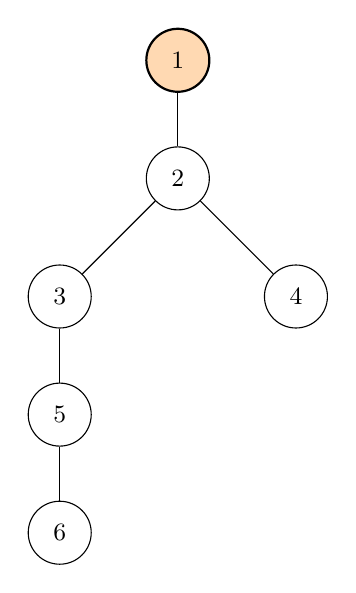
\begin{tikzpicture}[
    vertex/.style={circle, draw, minimum size=8mm, font=\small},
    start/.style={circle, draw, fill=orange!30, thick, minimum size=8mm, font=\small}
]

% Nodes
\node[start] (1) at (0,0) {1};
\node[vertex] (2) at (0,-1.5) {2};
\node[vertex] (3) at (-1.5,-3) {3};
\node[vertex] (4) at (1.5,-3) {4};
\node[vertex] (5) at (-1.5,-4.5) {5};
\node[vertex] (6) at (-1.5,-6) {6};

% Edges
\draw (1) -- (2);
\draw (2) -- (3);
\draw (2) -- (4);
\draw (3) -- (5);
\draw (5) -- (6);

\end{tikzpicture}

\vspace{2mm}
예제 출력: \textbf{6}

\end{frame}

\begin{frame}{트리의 높이}

\centering

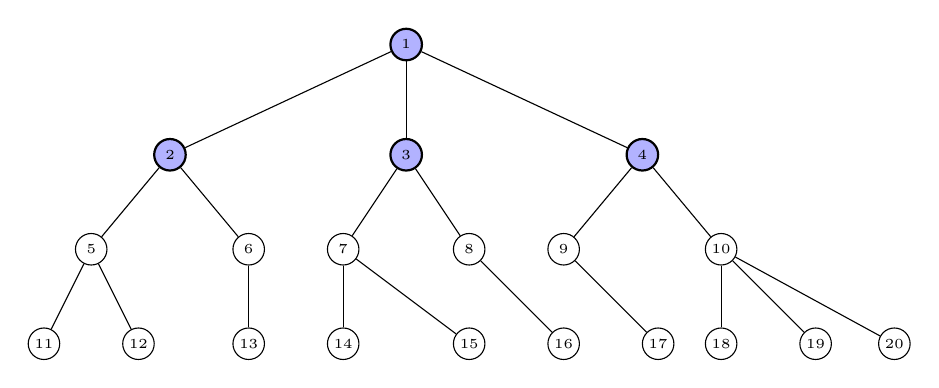
\begin{tikzpicture}[
    every node/.style={circle, draw, minimum size=4mm, inner sep=0pt, font=\tiny},
    high/.style={circle, draw, fill=blue!30, thick, minimum size=4mm, inner sep=0pt, font=\tiny}
]

% ----- 높이 0 -----
\node[high] (1) at (0,0) {1};

% ----- 높이 1 -----
\node[high] (2) at (-3,-1.4) {2};
\node[high] (3) at (0,-1.4) {3};
\node[high] (4) at (3,-1.4) {4};

% ----- 높이 2 -----
\node (5)  at (-4,-2.6) {5};
\node (6)  at (-2,-2.6) {6};
\node (7)  at (-0.8,-2.6) {7};
\node (8)  at (0.8,-2.6) {8};
\node (9)  at (2,-2.6) {9};
\node (10) at (4,-2.6) {10};

% ----- 높이 3 -----
\node (11) at (-4.6,-3.8) {11};
\node (12) at (-3.4,-3.8) {12};
\node (13) at (-2,-3.8) {13};
\node (14) at (-0.8,-3.8) {14};
\node (15) at (0.8,-3.8) {15};
\node (16) at (2,-3.8) {16};
\node (17) at (3.2,-3.8) {17};
\node (18) at (4,-3.8) {18};
\node (19) at (5.2,-3.8) {19};
\node (20) at (6.2,-3.8) {20};

% ----- 간선 -----

\draw (1)--(2);
\draw (1)--(3);
\draw (1)--(4);

\draw (2)--(5);
\draw (2)--(6);
\draw (3)--(7);
\draw (3)--(8);
\draw (4)--(9);
\draw (4)--(10);

\draw (5)--(11);
\draw (5)--(12);
\draw (6)--(13);
\draw (7)--(14);
\draw (7)--(15);
\draw (8)--(16);
\draw (9)--(17);
\draw (10)--(18);
\draw (10)--(19);
\draw (10)--(20);

\end{tikzpicture}

\vspace{2mm}
\small
높이가 2 이상인 정점

\end{frame}

\setproblem{19542}


\begin{frame}[fragile, allowframebreaks]{원찬혁 소스 코드}
\inputminted{java}{\prob/Chanhyeok.java}
\end{frame}

\begin{frame}[fragile, allowframebreaks]{정의찬 소스 코드}
\inputminted{java}{\prob/Uichan.java}
\end{frame}

\begin{frame}[fragile, allowframebreaks]{손현준 소스 코드}
\inputminted{java}{\prob/Hyeonjun.java}
\end{frame}

\begin{frame}[fragile, allowframebreaks]{서민종 소스 코드}
\inputminted{java}{\prob/Minjong.java}
\end{frame}

\begin{frame}[fragile, allowframebreaks]{임건애 소스 코드}
\inputminted{java}{\prob/Keonae.java}
\end{frame}

\begin{frame}[fragile, allowframebreaks]{김시온 소스 코드}
\inputminted{java}{\prob/Sion.java}
\end{frame}
